\documentclass[12pt,a4paper]{report}
% Packages
\usepackage[utf8]{inputenc}
\usepackage[T1]{fontenc}
\usepackage{amsmath}
\usepackage{amssymb}
\usepackage{graphicx}
\usepackage{booktabs}
\usepackage{array}
\usepackage{hyperref}
\usepackage{listings}
\usepackage{xcolor}
\usepackage{tikz}
\usepackage{caption}
\usepackage{subcaption}
\usepackage{multirow}
\usepackage{tabularx}
\usepackage{float}
\usepackage[margin=2cm]{geometry}
\usepackage{helvet}
\renewcommand{\familydefault}{\sfdefault}
\usepackage{titlesec}
\usetikzlibrary{positioning,shapes.geometric,arrows.meta}

% Chapter formatting (no "Chapter X" prefix, just the title)
\titleformat{\chapter}[display]
  {\normalfont\Large\bfseries\centering}
  {Chapter \thechapter}{0pt}{\LARGE}
\titlespacing*{\chapter}{0pt}{-20pt}{20pt}

% Section formatting
\titleformat{\section}{\normalfont\large\bfseries}{\thesection}{0.5em}{}
\titleformat{\subsection}{\normalfont\normalsize\bfseries}{\thesubsection}{0.5em}{}
\titleformat{\subsubsection}{\normalfont\normalsize\itshape}{\thesubsubsection}{0.5em}{}

% Dark theme code listing styles
\definecolor{codebg}{RGB}{40,42,54}
\definecolor{codecomment}{RGB}{98,114,164}
\definecolor{codestring}{RGB}{241,250,140}
\definecolor{codekeyword}{RGB}{255,121,198}
\definecolor{codenumber}{RGB}{189,147,249}
\definecolor{codetext}{RGB}{248,248,242}
\definecolor{codegreen}{RGB}{80,250,123}

\lstdefinestyle{codestyle}{
    basicstyle=\ttfamily\footnotesize\color{codetext},
    keywordstyle=\color{codekeyword}\bfseries,
    commentstyle=\color{codecomment}\itshape,
    stringstyle=\color{codestring},
    numberstyle=\tiny\color{codenumber},
    breaklines=true,
    frame=single,
    backgroundcolor=\color{codebg},
    rulecolor=\color{codebg},
    numbers=left,
    numbersep=8pt,
    xleftmargin=15pt,
    framexleftmargin=15pt,
    showstringspaces=false
}

\lstdefinestyle{bashstyle}{
    language=bash,
    basicstyle=\ttfamily\footnotesize\color{codetext},
    keywordstyle=\color{codekeyword},
    commentstyle=\color{codecomment},
    stringstyle=\color{codestring},
    breaklines=true,
    frame=single,
    backgroundcolor=\color{codebg},
    rulecolor=\color{codebg},
    showstringspaces=false
}

\lstdefinestyle{pythonstyle}{
    language=Python,
    basicstyle=\ttfamily\footnotesize\color{codetext},
    keywordstyle=\color{codekeyword}\bfseries,
    commentstyle=\color{codecomment}\itshape,
    stringstyle=\color{codestring},
    breaklines=true,
    frame=single,
    backgroundcolor=\color{codebg},
    rulecolor=\color{codebg},
    showstringspaces=false,
    morekeywords={self,True,False,None}
}

\lstdefinestyle{cppstyle}{
    language=C++,
    basicstyle=\ttfamily\footnotesize\color{codetext},
    keywordstyle=\color{codekeyword}\bfseries,
    commentstyle=\color{codecomment}\itshape,
    stringstyle=\color{codegreen},
    breaklines=true,
    frame=single,
    backgroundcolor=\color{codebg},
    rulecolor=\color{codebg},
    numbers=left,
    numberstyle=\tiny\color{codenumber},
    numbersep=8pt,
    xleftmargin=15pt,
    framexleftmargin=15pt,
    showstringspaces=false,
    morekeywords={int,void,class,public,private,return,if,for,while,break}
}

% Hyperref setup
\hypersetup{
    colorlinks=true,
    linkcolor=blue,
    citecolor=blue,
    urlcolor=blue
}

% Header and footer setup
\usepackage{fancyhdr}
\setlength{\headheight}{14.5pt}
\addtolength{\topmargin}{-2.5pt}
\pagestyle{fancy}
\fancyhf{}
\fancyhead[L]{William Park}
\fancyhead[R]{Survey on Parallel Subgraph Matching}
\fancyfoot[R]{\thepage}
\renewcommand{\headrulewidth}{0.4pt}
\renewcommand{\footrulewidth}{0pt}

% Also apply to chapter pages
\fancypagestyle{plain}{
    \fancyhf{}
    \fancyhead[L]{William Park}
    \fancyhead[R]{Survey on Parallel Subgraph Matching}
    \fancyfoot[R]{\thepage}
    \renewcommand{\headrulewidth}{0.4pt}
}

% Start page numbering at 37 and chapter at 5
\setcounter{page}{37}
\setcounter{chapter}{4}

\begin{document}

%==============================================================================
\chapter{Benchmarking Framework Architecture}
\label{ch:framework}
%==============================================================================

A critical challenge in comparative evaluation of parallel subgraph isomorphism algorithms is the heterogeneity of implementations: each algorithm employs different input formats, command-line interfaces, output conventions, and configuration mechanisms. To enable fair and consistent comparison, we developed a unified benchmarking framework based on the \emph{Controller-Adapter} design pattern.

\section{Design Pattern: Controller-Adapter Architecture}

The Controller-Adapter pattern provides a clean abstraction layer between the benchmarking logic and algorithm-specific implementation details. This architecture comprises three principal components:

\begin{enumerate}
    \item \textbf{Master Controller}: A central orchestration module that coordinates experiment execution, manages configuration, and aggregates results.
    \item \textbf{Unified Interface}: An abstract specification defining the contract that all algorithm adapters must implement.
    \item \textbf{Algorithm Adapters}: Concrete implementations that wrap each algorithm's binary executable and translate between the unified interface and algorithm-specific conventions.
\end{enumerate}

Figure~\ref{fig:adapter-architecture} illustrates the architectural hierarchy.

\begin{figure}[htbp]
\centering
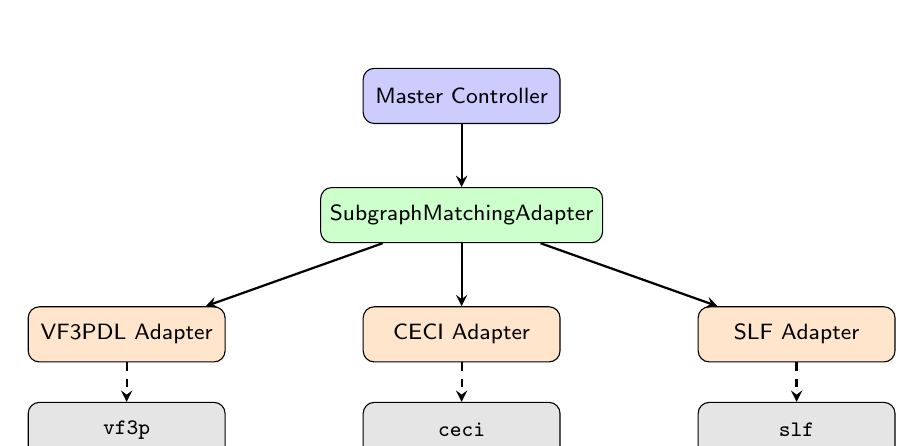
\begin{tikzpicture}[
    node distance=0.8cm,
    box/.style={rectangle, draw, rounded corners, minimum width=2.5cm, minimum height=0.7cm, align=center, font=\footnotesize},
    arrow/.style={->, >=stealth, thick}
]
% Controller
\node[box, fill=blue!20] (ctrl) {Master Controller};
% Interface
\node[box, fill=green!20, below=of ctrl] (iface) {SubgraphMatchingAdapter};
% Adapters
\node[box, fill=orange!20, below left=0.8cm and 1.2cm of iface] (vf3) {VF3PDL Adapter};
\node[box, fill=orange!20, below=of iface] (ceci) {CECI Adapter};
\node[box, fill=orange!20, below right=0.8cm and 1.2cm of iface] (slf) {SLF Adapter};
% Binaries
\node[box, fill=gray!20, below=0.5cm of vf3] (vf3bin) {\texttt{vf3p}};
\node[box, fill=gray!20, below=0.5cm of ceci] (cecibin) {\texttt{ceci}};
\node[box, fill=gray!20, below=0.5cm of slf] (slfbin) {\texttt{slf}};
% Arrows
\draw[arrow] (ctrl) -- (iface);
\draw[arrow] (iface) -- (vf3);
\draw[arrow] (iface) -- (ceci);
\draw[arrow] (iface) -- (slf);
\draw[arrow, dashed] (vf3) -- (vf3bin);
\draw[arrow, dashed] (ceci) -- (cecibin);
\draw[arrow, dashed] (slf) -- (slfbin);
\end{tikzpicture}
\caption{Controller-Adapter architecture. Solid arrows: method calls; dashed arrows: subprocess execution.}
\label{fig:adapter-architecture}
\end{figure}

\section{Standardising Input Format}

Table~\ref{tab:formats} summarises the input format requirements for each algorithm.

\begin{table}[htbp]
\centering
\caption{Input format specifications for evaluated algorithms.}
\label{tab:formats}
\begin{tabular}{llll}
\toprule
\textbf{Algorithm} & \textbf{Format} & \textbf{Type} & \textbf{Structure} \\
\midrule
VF3P & VF3/Adjacency & Text & Adjacency list \\
CECI & HKU/Edge List & Text & Edge list with header \\
SLF & VF3/Adjacency & Text & Adjacency list \\
\bottomrule
\end{tabular}
\end{table}

\paragraph{VF3/Adjacency Format.}
The VF3 format represents graphs as adjacency lists. The first line specifies the vertex count, followed by vertex definitions (ID and label), then for each vertex, the edge count and incident edges:

\begin{lstlisting}[style=bashstyle]
8                    # Number of vertices
0 1                  # Vertex 0, label 1
1 1                  # Vertex 1, label 1
5                    # Vertex 0 has 5 edges
0 1                  # Edge 0 -> 1
0 2                  # Edge 0 -> 2
\end{lstlisting}

\paragraph{HKU/Edge List Format.}
The HKU format employs an explicit edge list representation:

\begin{lstlisting}[style=bashstyle]
t # 0                # Graph identifier
v 0 1                # Vertex 0, label 1
v 1 1                # Vertex 1, label 1
e 0 1 0              # Edge from 0 to 1, label 0
e 0 2 0              # Edge from 0 to 2, label 0
\end{lstlisting}

\section{Adapter Implementation}

Each adapter implements the \texttt{SubgraphMatchingAdapter} abstract base class:

\begin{lstlisting}[style=pythonstyle]
class SubgraphMatchingAdapter(ABC):
    @abstractmethod
    def run(self, query_path: str, data_path: str,
            threads: int, timeout: int,
            solution_limit: int) -> BenchmarkResult:
        """Execute subgraph matching."""
        pass

    @abstractmethod
    def get_graph_format(self) -> str:
        """Return expected input format identifier."""
        pass
\end{lstlisting}

\section{Master Controller Operation}

The master controller implements experiment orchestration through nested iteration over the experimental parameter space:

\begin{lstlisting}[style=pythonstyle]
for algorithm in algorithms:
    adapter = get_adapter(algorithm)
    for dataset in datasets:
        for query in queries[dataset]:
            for threads in thread_counts:
                result = adapter.run(
                    query, data_graph[dataset],
                    threads, TIMEOUT, LIMIT)
                append_to_csv(result)
\end{lstlisting}

\section{Standardised Output Format}

All adapters produce results conforming to a unified CSV schema:

\begin{lstlisting}[style=bashstyle]
Algorithm,Dataset,Query,Threads,Time_s,Solutions,Memory_MB,Status
VF3-O,enron,query_dense_8v_1,8,0.234,15420,128.5,SUCCESS
CECI,enron,query_dense_8v_1,8,0.187,15420,145.2,SUCCESS
SLF,enron,query_dense_8v_1,8,0.156,15420,112.8,SUCCESS
\end{lstlisting}

%==============================================================================
\chapter{Experimental Setup}
\label{ch:setup}
%==============================================================================

\section{Hardware Environment}

\paragraph{Primary Server.}
All experiments were conducted on TODS1 (\texttt{tods1.cse.unsw.edu.au}), a shared server in the UNSW CSE department with the following specifications:

\begin{itemize}
    \item \textbf{CPUs}: 96 logical cores (48 physical cores with hyperthreading)
    \item \textbf{Architecture}: 2 NUMA nodes (Node 0: cores 0--23, 48--71; Node 1: cores 24--47, 72--95)
    \item \textbf{Memory}: 502 GB shared RAM
\end{itemize}

\paragraph{Development Environment.}
Local testing and development was performed on a MacBook Air M2 (8GB RAM).

\section{Software Environment}

\begin{itemize}
    \item \textbf{Language}: C++
    \item \textbf{Parallelisation}: OpenMP
    \item \textbf{Compiler}: GCC (standard Linux toolchain on Ubuntu)
    \item \textbf{Build System}: Make
\end{itemize}

\section{Experimental Parameters}

Table~\ref{tab:parameters} summarises the experimental configuration.

\begin{table}[htbp]
\centering
\caption{Experimental parameters.}
\label{tab:parameters}
\begin{tabular}{ll}
\toprule
\textbf{Parameter} & \textbf{Value} \\
\midrule
Thread counts & 1, 2, 4, 8, 16, 32, 64 \\
Match limit ($K$) & 50 million (500M for select tests) \\
Timeout & 600 seconds (10 minutes) \\
\bottomrule
\end{tabular}
\end{table}

\section{Datasets}

Table~\ref{tab:datasets} describes the graph datasets used in our evaluation.

\begin{table}[htbp]
\centering
\caption{Dataset characteristics.}
\label{tab:datasets}
\begin{tabular}{llrr}
\toprule
\textbf{Dataset} & \textbf{Type} & \textbf{Vertices} & \textbf{Edges} \\
\midrule
ENRON & Email network & $\sim$37K & $\sim$368K \\
DBLP & Collaboration network & $\sim$317K & $\sim$1M \\
LiveJournal & Social network & $\sim$4M & $\sim$35M \\
RoadNet-CA & Road network & $\sim$2M & $\sim$5.5M \\
\bottomrule
\end{tabular}
\end{table}

\section{Query Patterns}

Query patterns were generated with the following characteristics:

\begin{itemize}
    \item \textbf{Densities}: Sparse, Dense
    \item \textbf{Sizes}: 8, 16, 24, 32 vertices
    \item \textbf{Format}: 5 queries per (density $\times$ size) combination
\end{itemize}

\section{Algorithms Compared}

Table~\ref{tab:algorithms} summarises the algorithms evaluated in this study.

\begin{table}[htbp]
\centering
\caption{Evaluated algorithms and their parallelisation strategies.}
\label{tab:algorithms}
\begin{tabular}{lp{4cm}}
\toprule
\textbf{Algorithm} & \textbf{Parallelisation Strategy} \\
\midrule
VF3PDL & Domain decomposition with descendant limit \\
SLF & Passive work sharing with depth priority \\
CECI & Index-based intersection \\
\bottomrule
\end{tabular}
\end{table}

\section{Research Questions}

This evaluation addresses three research questions:

\begin{enumerate}
    \item[\textbf{RQ1}:] How do parallel subgraph matching algorithms scale, and what limits their speedup?
    \item[\textbf{RQ2}:] How do graph density and topology affect the relative performance of traversal-based (SLF/VF3) versus index-based (CECI) algorithms?
    \item[\textbf{RQ3}:] Is there a fundamental tradeoff between pruning effectiveness and parallel scalability?
\end{enumerate}

%==============================================================================
\chapter{Experimental Results}
\label{ch:results}
%==============================================================================

%------------------------------------------------------------------------------
\section{Research Question 1: Parallel Scaling Behaviour}
\label{sec:rq1}
%------------------------------------------------------------------------------

This section addresses Research Question 1: How do parallel subgraph matching algorithms scale, and what limits their speedup? The analysis evaluates three algorithms: VF3 (specifically the VF3PDL implementation), CECI, and SLF.

Parallel speedup is formally defined as $S_p = T_1 / T_p$, where $T_1$ is sequential execution time and $T_p$ is parallel execution time on $p$ processors. The theoretical upper bound establishes that $T_1 \leq p \cdot T_p$, implying linear speedup ($S_p = p$) as the maximum achievable under ideal conditions. Superlinear speedup ($S_p > p$) can occur in search problems due to work anomalies, where parallel exploration collectively avoids unproductive regions.

\subsection{Memory Constraints and Scalability Limits}

\begin{figure}[htbp]
\centering
\includegraphics[width=0.9\textwidth]{rq1_memory_scaling.png}
\caption{Memory consumption scaling from 1 to 64 threads across datasets.}
\label{fig:rq1-memory}
\end{figure}

This experiment examines the memory consumption of each algorithm as thread counts increase from 1 to 64. The results indicate a significant divergence in resource management strategies between traversal-based and index-based approaches.

VF3 exhibits a strictly linear increase in memory consumption relative to thread count. On the RoadNet dataset with dense 8-vertex queries, memory usage increases from approximately 1.6 GB at 1 thread to 43 GB at 64 threads, representing a 27-fold increase. The growth is even more pronounced on DBLP, escalating from 272 MB to 10.3 GB (38-fold increase). This suggests that VF3 allocates deep copies of state for each worker, creating a hard scalability limit on memory-constrained systems.

CECI, in contrast, maintains a constant memory footprint regardless of thread count. Usage remains stable at approximately 125 MB for RoadNet and 63 MB for DBLP across all thread counts. This indicates that CECI threads operate on a shared, read-only index structure without significant per-thread allocation.

SLF demonstrates moderate linear growth, with memory usage on RoadNet rising from approximately 760 MB to 4 GB (a 5.3-fold increase). This suggests an optimised sharing mechanism that incurs significantly lower overhead than VF3 while still requiring some per-thread state.

\subsection{Superlinear Scaling Anomalies (8-Vertex Queries)}

\begin{figure}[htbp]
\centering
\includegraphics[width=0.9\textwidth]{rq1_superlinear.png}
\caption{Superlinear scaling anomalies observed on 8-vertex queries.}
\label{fig:rq1-superlinear}
\end{figure}

This section analyses scaling efficiency, defined as the ratio of throughput at thread count $t$ to throughput at 1 thread, across varying graph topologies. The data highlights contrasting behaviours driven by search space characteristics and synchronisation overhead.

On 16-vertex sparse queries, VF3 demonstrates robust scalability, achieving speedups of approximately 25x at 64 threads on Enron and 12x on DBLP. SLF displays dataset-dependent performance, achieving near-linear scaling on DBLP (26x speedup) but degrading on the sparse Enron dataset (0.7x).

With smaller 8-vertex queries, significant superlinear speedups are observed. VF3 achieves a speedup of 78.6x on Enron (sparse 8v), while SLF achieves 117x on DBLP (dense 8v). These values exceed the theoretical linear bound of 64x, representing efficiencies of 123\% and 183\% respectively. This behaviour is consistent with ``search anomalies'' documented in parallel depth-first search literature, where parallel workers bypass ineffective search branches that would otherwise delay single-threaded execution. The irregular structure of subgraph isomorphism search spaces makes them particularly susceptible to such anomalies.

CECI exhibits the opposite pattern, demonstrating negative scalability ($S_p < 1$) across all tested workloads. Performance decreases to 0.10x on Enron and remains below the break-even threshold across all datasets: 0.58x on DBLP, 0.69x on RoadNet, and 0.96x on LiveJournal. This violation of expected scaling behaviour indicates that synchronisation overhead on the shared index structure exceeds the computational work distributed per thread. The atomic operations required to maintain index consistency impose costs that grow with thread count, effectively negating parallel gains.

\subsection{Standard Scaling Behaviour (16-Vertex Queries)}

\begin{figure}[htbp]
\centering
\includegraphics[width=0.9\textwidth]{rq1_speedup_curves.png}
\caption{Thread scaling behaviour on 16-vertex queries across datasets.}
\label{fig:rq1-speedup-curves}
\end{figure}

This section analyses scaling efficiency, defined as the ratio of throughput at thread count $t$ to throughput at 1 thread, for standard 16-vertex workloads. Figure~\ref{fig:rq1-speedup-curves} presents the scaling curves for all four datasets, enabling direct comparison of algorithmic behaviour across diverse graph topologies.

VF3 demonstrates consistent scalability across sparse datasets, achieving a speedup of approximately 25x at 64 threads on Enron and 12x on DBLP. The scaling curve remains positive throughout, indicating effective load balancing across workers.

CECI exhibits the opposite behaviour, demonstrating negative scalability across all tested configurations. Performance decreases to 0.10x on Enron, representing a 90\% performance loss relative to single-threaded execution, and remains below 1x across all tested datasets (0.58x on DBLP, 0.69x on RoadNet). This degradation suggests that the overhead of atomic synchronisation outweighs the benefits of parallel execution for these workloads.

SLF displays dataset-dependent performance. On DBLP, it achieves near-linear scaling with a 26x speedup, yet on the sparse Enron dataset, performance degrades to 0.7x. This dichotomy suggests that stream-based filtering requires sufficient graph density to amortise the coordination overhead.

\subsection{Aggregate Parallel Efficiency at High Concurrency}

\begin{figure}[htbp]
\centering
\includegraphics[width=0.9\textwidth]{rq1_speedup_bar.png}
\caption{Maximum speedup achieved at 64 threads across all configurations.}
\label{fig:rq1-speedup-bar}
\end{figure}

This analysis summarises the maximum speedup achieved at 64 threads, isolating the relative efficiency of each algorithm under high parallelism.

VF3 emerges as the most scalable algorithm, consistently achieving positive scaling across all configurations. Speedups range from 3.0x on LiveJournal sparse queries to 56.4x on RoadNet dense queries, with a notable peak of 41.4x on Enron dense. This suggests that VF3's task-based architecture effectively partitions the search space, minimising contention between workers.

CECI performance at 64 threads is consistently below the break-even threshold of 1x. Speedups range from 0.10x to 0.96x, with no instance of positive scaling observed across any dataset or query configuration. These results suggest that the query execution phase of CECI is predominantly sequential, limiting the benefit of additional threads regardless of available parallelism.

SLF achieves substantial speedups on dense graphs, reaching 27x on DBLP dense and 26x on DBLP sparse. However, on the sparse Enron dataset, it falls below the break-even threshold at 0.7x. This reinforces that stream-based filtering requires sufficient graph density to be effective.

Taken together, these findings demonstrate that the limits to parallel speedup are algorithm-specific. VF3 is primarily constrained by memory availability, reaching 72 GB at 64 threads on LiveJournal. CECI is limited by synchronisation overhead inherent to its shared index structure. SLF offers a middle ground, achieving strong scaling on dense graphs while remaining sensitive to sparse topologies.

%------------------------------------------------------------------------------
\section{Research Question 2: Graph Density and Topology Effects}
\label{sec:rq2}
%------------------------------------------------------------------------------

This section addresses Research Question 2: How do graph density and topology affect the relative performance of traversal-based (SLF/VF3) versus index-based (CECI) algorithms? The analysis synthesises data from performance heatmaps, density comparisons, and scale-based evaluations to establish the relationship between graph structure and algorithmic efficacy.

\subsection{The Density Crossover Effect}

\begin{figure}[htbp]
\centering
\includegraphics[width=0.9\textwidth]{rq2_density_effect.png}
\caption{The density crossover effect: performance inversion between sparse and dense queries.}
\label{fig:rq2-density}
\end{figure}

A comparative analysis of sparse versus dense 16-vertex queries reveals a fundamental performance inversion dictated by graph density.

In sparse query scenarios, the index-based algorithm (CECI) consistently outperforms or remains competitive with traversal-based alternatives. On the LiveJournal dataset, CECI achieves approximately 0.5 million EPS, significantly surpassing SLF (approximately 0.1 million EPS) and VF3 (below 0.01 million EPS). On RoadNet, CECI is the sole viable candidate, achieving roughly 3 million EPS while traversal-based methods achieve throughput below $10^3$ EPS.

As query density increases, a distinct crossover occurs. On LiveJournal with dense 16-vertex queries, SLF performance increases to approximately 13 million EPS, representing a 130-fold improvement compared to its sparse performance. CECI shows no comparable gain, remaining relatively static or degrading. Similarly, on DBLP with dense queries, SLF maintains a lead with approximately 17 million EPS compared to CECI's 8 million EPS.

This inversion suggests that increased graph density facilitates traversal-based algorithms by providing more high-degree vertices for effective candidate pruning. Index-based approaches such as CECI incur quadratic filtering costs on dense neighbourhoods, which potentially negates the benefits of indexing.

\subsection{Topological Sensitivity and Planar Graph Limitations}

\begin{figure}[htbp]
\centering
\includegraphics[width=0.9\textwidth]{rq2_scale_effect.png}
\caption{Performance variation across graph scales and topologies.}
\label{fig:rq2-scale}
\end{figure}

This experiment isolates the impact of graph topology by comparing performance across datasets of increasing scale and varying structural properties using sparse 16-vertex queries. Figure~\ref{fig:rq2-scale} visualises this relationship, plotting EPS against graph size to reveal how each algorithm responds to increasing scale.

The RoadNet dataset represents a planar, mesh-like topology characterised by a lack of high-degree nodes. On this dataset, the performance gap is substantial: CECI achieves approximately 3 million EPS, whereas VF3 and SLF exhibit near-zero performance (below $10^3$ EPS).

The failure of VF3 and SLF on RoadNet indicates that traversal heuristics rely heavily on degree heterogeneity to guide the search. In planar graphs where degree distribution is narrow and uniform, these heuristics fail to prune the search space effectively, leading to excessive exploration or timeouts.

CECI's success on RoadNet demonstrates the robustness of index-based approaches on planar graphs. By constructing a global index, CECI can locate rare embeddings directly without traversing the sparse search region of uniform low-degree nodes. It should be noted, however, that the classification of RoadNet as ``planar'' is based on its known road network structure rather than formal planarity testing.

\subsection{Global Performance Landscape}

\begin{figure}[htbp]
\centering
\includegraphics[width=0.9\textwidth]{rq2_winner_heatmap.png}
\caption{Optimal algorithm selection heatmap across dataset-query combinations at 64 threads.}
\label{fig:rq2-heatmap}
\end{figure}

A comprehensive heatmap identifying the optimal algorithm for each dataset-query combination at 64 threads establishes clear zones of dominance for each algorithmic class.

CECI emerges as the dominant algorithm for sparse queries, securing the top position on RoadNet (all queries), LiveJournal (all sparse queries), and Enron (sparse 16v and 32v). This suggests its suitability for low-selectivity tasks where minimising search operations is critical.

SLF demonstrates superior performance for dense workloads, achieving optimal results across the DBLP dataset (5 out of 6 configurations) and LiveJournal (dense 8v and 16v). On LiveJournal dense 16v, SLF achieves 13.3 million EPS compared to CECI's substantially lower throughput.

VF3 appears as a specialised solution, achieving optimal performance only on Enron dense 8v (11.0 million EPS). This suggests that while VF3's task-based parallelism is effective, it generally lacks the pruning power to compete with SLF or CECI on larger or more complex graphs.

These results demonstrate that no single algorithm dominates across all configurations. Effective algorithm selection requires consideration of graph topology: CECI for sparse and planar graphs, SLF for dense scale-free graphs, and VF3 for small-scale dense queries where memory constraints permit.

%------------------------------------------------------------------------------
\section{Research Question 3: Pruning vs Scalability Tradeoff}
\label{sec:rq3}
%------------------------------------------------------------------------------

This section addresses Research Question 3: Is there a fundamental tradeoff between pruning effectiveness and parallel scalability? By analysing single-thread performance against multi-threaded speedups, the results establish a clear inverse relationship between the sophistication of sequential pruning and the capacity for parallel scaling.

\subsection{The Pruning-Scalability Inversion}

\begin{figure}[htbp]
\centering
\includegraphics[width=0.9\textwidth]{rq3_grouped_bar.png}
\caption{Cross-algorithm comparison of single-thread performance versus parallel speedup.}
\label{fig:rq3-grouped}
\end{figure}

A cross-algorithm comparison reveals a clear dichotomy between algorithms optimised for pruning and those optimised for scaling.

CECI represents the extreme of pruning effectiveness. At 1 thread, it achieves massive throughput (64 million EPS) by using an index to aggressively filter candidates before search. However, this pre-processing comes at a cost: when scaled to 64 threads, CECI exhibits a speedup of just 0.33x---a performance regression. This suggests that the shared data structures required for effective pruning create synchronisation bottlenecks that inhibit parallelism.

Conversely, VF3 represents the extreme of scalability. Its single-thread performance is relatively low (119K EPS) due to minimal pre-filtering during traversal. However, this independence allows it to scale substantially, achieving a speedup of 28x at 64 threads. The absence of complex shared state allows threads to partition the search space without contention.

SLF occupies the middle ground, offering moderate pruning (540K EPS at 1 thread) and moderate scalability (12x speedup). This suggests that stream-based filtering provides a compromise, avoiding the severe locking of index-based approaches while achieving better pruning than raw traversal.

These findings point to a quantifiable cost associated with algorithmically ``sophisticated'' approaches: the more effective an algorithm is at sequential pruning, the harder it becomes to parallelise the remaining work effectively.

\subsection{The Amdahl's Law Bottleneck}

\begin{figure}[htbp]
\centering
\includegraphics[width=0.9\textwidth]{rq3_ceci_breakdown.png}
\caption{CECI filter vs enumeration phase breakdown across query configurations.}
\label{fig:rq3-breakdown}
\end{figure}

To explain the mechanism behind this tradeoff, the execution time breakdown of CECI was analysed across varying graph densities.

Amdahl's Law provides the theoretical framework for understanding these limits. For a program with sequential fraction $s$, maximum speedup on $n$ processors is bounded by:

\begin{equation}
S_{\max} = \frac{n}{1 + (n-1)s}
\end{equation}

As $n \to \infty$, this converges to $1/s$, establishing an absolute ceiling independent of available parallelism.

On dense graphs such as LiveJournal, execution is dominated by the filtering phase. For 8v, 16v, and 32v queries, the pruning phase consumes between 99\% and 100\% of total execution time ($s \approx 0.99$). Substituting into Amdahl's formula with $n = 64$ processors:

\begin{equation}
S_{\max} = \frac{64}{1 + (63)(0.99)} = \frac{64}{63.37} \approx 1.01
\end{equation}

This theoretical ceiling of 1.01x precisely matches our empirical observation of 0.96x speedup for CECI on LiveJournal---the slight underperformance attributable to synchronisation overhead not captured in the idealized model.

The pattern differs markedly on sparse graphs. On Enron (8v), the pruning phase consumes only approximately 3\% of execution time ($s = 0.03$), leaving 97\% for the parallel enumeration phase:

\begin{equation}
S_{\max} = \frac{64}{1 + (63)(0.03)} = \frac{64}{2.89} \approx 22.1
\end{equation}

This explains why CECI remains viable on sparse datasets but exhibits degraded performance on dense graphs.

Taken together, these results demonstrate that the tradeoff is structural: aggressive index-based pruning shifts the computational burden from the parallelisable enumeration phase to the inherently sequential filtering phase. For dense graphs, this shift is detrimental to scalability. However, this analysis assumes that CECI's filtering phase cannot be parallelised; future implementations achieving partial parallelisation of index construction may alter this tradeoff.

\subsection{Absolute Performance Impact}

\begin{figure}[htbp]
\centering
\includegraphics[width=0.9\textwidth]{rq3_speedup.png}
\caption{Absolute performance comparison showing the ``head start'' effect.}
\label{fig:rq3-speedup}
\end{figure}

While scalability metrics favour VF3, absolute performance metrics reveal a more nuanced picture of the value of pruning.

Despite its poor scaling, CECI's single-thread performance is sufficiently high (64M EPS) that even after degrading to 10M EPS at 64 threads, it still outperforms VF3's best parallel result (4M EPS) in this aggregate view. This ``head start'' effect demonstrates that raw throughput and scalability represent distinct, sometimes competing, objectives.

VF3 starts at a substantial disadvantage (0.1M EPS) but closes the gap significantly through parallelism, reaching 4M EPS. While it does not overtake CECI in this aggregate view, the trajectory suggests that the minimally-pruned but scalable approach could eventually surpass the aggressively-pruned but sequential approach on systems with higher core counts, particularly if the negative scaling trend continues.

These findings suggest a fundamental tradeoff between pruning effectiveness and parallel scalability. For single-threaded or low-parallelism environments, index-based approaches such as CECI remain optimal. For massively parallel systems, traversal-based approaches such as VF3 offer superior scaling despite lower baseline performance.

%==============================================================================
\chapter{Synthetic Validation}
\label{ch:synthetic}
%==============================================================================

To validate the findings from real-world datasets and isolate the effects of graph topology on algorithm performance, we conducted controlled experiments on synthetic graphs with known structural properties. This validation complements the real-world evaluation by removing confounding factors such as label distributions, community structures, and dataset-specific anomalies.

%------------------------------------------------------------------------------
\section{Synthetic Graph Generation}
\label{sec:synthetic-generation}
%------------------------------------------------------------------------------

Two well-established random graph models were employed to generate synthetic datasets:

\paragraph{Erdős-Rényi Model $G(n,p)$.}
The Erdős-Rényi model generates graphs by connecting each pair of $n$ vertices independently with probability $p$. This produces uniformly random graphs with binomial degree distributions and no inherent community structure or degree heterogeneity. The lack of exploitable structure makes ER graphs a rigorous test for pruning-based algorithms.

\paragraph{Barabási-Albert Model.}
The Barabási-Albert (BA) model generates scale-free graphs through preferential attachment: new vertices connect preferentially to existing high-degree vertices. This produces power-law degree distributions with hub structures, more closely resembling real-world social and biological networks.

Table~\ref{tab:synthetic-graphs} summarises the generated graph configurations.

\begin{table}[htbp]
\centering
\caption{Synthetic graph configurations. All graphs contain 50,000 vertices.}
\label{tab:synthetic-graphs}
\begin{tabular}{llrrl}
\toprule
\textbf{Model} & \textbf{Graph} & \textbf{Edges} & \textbf{Avg. Degree} & \textbf{Structure} \\
\midrule
Erdős-Rényi & er\_250k & 249,707 & 10.0 & Uniform random \\
Erdős-Rényi & er\_500k & 500,356 & 20.0 & Uniform random \\
Erdős-Rényi & er\_1m & 1,000,236 & 40.0 & Uniform random \\
Erdős-Rényi & er\_2m & 2,000,819 & 80.0 & Uniform random \\
Erdős-Rényi & er\_3m & 3,001,844 & 120.0 & Uniform random \\
\midrule
Barabási-Albert & ba\_50k & 49,999 & 2.0 & Scale-free (hubs) \\
Barabási-Albert & ba\_100k & 99,996 & 4.0 & Scale-free (hubs) \\
Barabási-Albert & ba\_250k & 249,975 & 10.0 & Scale-free (hubs) \\
Barabási-Albert & ba\_500k & 499,900 & 20.0 & Scale-free (hubs) \\
Barabási-Albert & ba\_750k & 749,775 & 30.0 & Scale-free (hubs) \\
\bottomrule
\end{tabular}
\end{table}

\paragraph{Query Patterns.}
Four query types were evaluated: sparse 8-vertex, dense 8-vertex, sparse 16-vertex, and dense 16-vertex patterns. This mirrors the real-world experimental configuration.

\paragraph{Experimental Parameters.}
All experiments used identical parameters to the real-world evaluation: $K$-limit of 500 million embeddings, timeout of 120 seconds, and 64 threads. This configuration enables direct comparison between synthetic and real-world results.

%------------------------------------------------------------------------------
\section{RQ1: Algorithm Performance on Synthetic Graphs}
\label{sec:synthetic-rq1}
%------------------------------------------------------------------------------

\begin{figure}[htbp]
\centering
\includegraphics[width=0.75\textwidth]{synthetic_rq1_comparison.png}
\caption{RQ1 Validation: Average algorithm performance across all synthetic graphs. CECI achieves 29.1M EPS, SLF 167K EPS, and VF3PDL 10.2K EPS.}
\label{fig:synthetic-rq1}
\end{figure}

Figure~\ref{fig:synthetic-rq1} presents the average throughput across all synthetic graph configurations. The results reveal a substantial performance disparity between index-based and traversal-based approaches. CECI maintains an average throughput of 29 million EPS across all configurations, while SLF achieves 167K EPS and VF3PDL is limited to approximately 10K EPS.

These results are consistent with the performance trends observed on real-world datasets, where CECI consistently achieved the highest throughput. However, the performance gap is significantly amplified in the synthetic environment. On real-world graphs, traversal-based algorithms typically lag CECI by one to two orders of magnitude; on synthetic graphs, this gap expands to nearly three orders of magnitude. This amplification suggests that traversal-based algorithms rely heavily on the structural properties present in real-world graphs, such as community structure and degree heterogeneity, to prune the search space effectively. When such structure is absent, their performance degrades disproportionately.

%------------------------------------------------------------------------------
\section{RQ2: Topology Effects on Erdős-Rényi and Barabási-Albert Graphs}
\label{sec:synthetic-rq2}
%------------------------------------------------------------------------------

\begin{figure}[htbp]
\centering
\includegraphics[width=0.85\textwidth]{synthetic_rq2_er.png}
\caption{RQ2 Validation: Algorithm performance on Erdős-Rényi $G(n,p)$ graphs. VF3PDL exhibits severe degradation (4,387 $\rightarrow$ 99 EPS) as graph size increases, while CECI maintains constant $\sim$30M EPS.}
\label{fig:synthetic-rq2-er}
\end{figure}

Figure~\ref{fig:synthetic-rq2-er} presents algorithm performance on Erdős-Rényi graphs, which exhibit uniform degree distributions and lack community structure. CECI maintains stable throughput of approximately 30 million EPS regardless of graph scale. SLF exhibits moderate degradation, with throughput dropping from 274K EPS on the smallest graph to 104K EPS on the largest, representing a 2.6-fold reduction. VF3PDL suffers severe degradation, with throughput falling from 4,387 EPS to just 99 EPS as graph size increases from 250K to 3M edges. This 44-fold reduction confirms that VF3PDL's pruning heuristics depend on discriminatory structural features to guide the search. In random graphs where local neighbourhoods are statistically uniform, these heuristics fail to prune effectively, forcing the algorithm into near-exhaustive exploration.

Table~\ref{tab:synthetic-er-sparse} provides detailed EPS values for sparse queries on ER graphs.

\begin{table}[htbp]
\centering
\caption{Sparse query performance on Erdős-Rényi graphs (EPS).}
\label{tab:synthetic-er-sparse}
\begin{tabular}{lrrr}
\toprule
\textbf{Graph} & \textbf{CECI} & \textbf{SLF} & \textbf{VF3PDL} \\
\midrule
er\_250k (250K edges) & 28,043,463 & 274,415 & 4,387 \\
er\_500k (500K edges) & 31,567,415 & 254,921 & 1,569 \\
er\_1m (1M edges) & 32,569,885 & 268,008 & 608 \\
er\_2m (2M edges) & 32,666,319 & 186,658 & 192 \\
er\_3m (3M edges) & 30,556,861 & 103,936 & 99 \\
\midrule
\textbf{Degradation} & 1.0$\times$ & 2.6$\times$ & \textbf{44$\times$} \\
\bottomrule
\end{tabular}
\end{table}

\begin{figure}[htbp]
\centering
\includegraphics[width=0.85\textwidth]{synthetic_rq2_ba.png}
\caption{RQ2 Validation: Algorithm performance on Barabási-Albert scale-free graphs. Hub structure provides marginally better pruning opportunities for VF3PDL compared to ER graphs.}
\label{fig:synthetic-rq2-ba}
\end{figure}

Figure~\ref{fig:synthetic-rq2-ba} presents results on Barabási-Albert graphs, which model scale-free networks with power-law degree distributions. The presence of hub vertices in BA graphs provides anchor points for traversal heuristics, enabling more effective pruning than on random graphs. CECI remains stable at 30-35 million EPS. VF3PDL shows improved resilience compared to the ER case, with throughput dropping from 133 to 12 EPS across the tested range. This 11-fold reduction, compared to the 44-fold reduction observed on ER graphs, indicates that hub structure partially compensates for the lack of community organisation. However, traversal-based throughput remains orders of magnitude lower than CECI, demonstrating that while hubs mitigate degradation, they do not eliminate the fundamental advantage of index-based enumeration.

Table~\ref{tab:synthetic-ba-sparse} provides detailed EPS values for sparse queries on BA graphs.

\begin{table}[htbp]
\centering
\caption{Sparse query performance on Barabási-Albert graphs (EPS).}
\label{tab:synthetic-ba-sparse}
\begin{tabular}{lrrr}
\toprule
\textbf{Graph} & \textbf{CECI} & \textbf{SLF} & \textbf{VF3PDL} \\
\midrule
ba\_50k (50K edges) & 34,507,994 & 143,507 & 133 \\
ba\_100k (100K edges) & 34,783,802 & 185,848 & 46 \\
ba\_250k (250K edges) & 35,432,489 & 300,630 & 30 \\
ba\_500k (500K edges) & 35,248,839 & 123,831 & 33 \\
ba\_750k (750K edges) & 35,653,158 & 131,180 & 12 \\
\midrule
\textbf{Degradation} & 1.0$\times$ & 2.3$\times$ & \textbf{11$\times$} \\
\bottomrule
\end{tabular}
\end{table}

%------------------------------------------------------------------------------
\section{RQ3: The Pruning-Structure Dependency}
\label{sec:synthetic-rq3}
%------------------------------------------------------------------------------

\begin{figure}[htbp]
\centering
\includegraphics[width=0.85\textwidth]{synthetic_er.png}
\caption{RQ3 Validation: Pruning (VF3PDL) vs parallel enumeration (CECI) on Erdős-Rényi graphs. The 5-order-of-magnitude performance gap demonstrates that pruning strategies fail without exploitable structure.}
\label{fig:synthetic-rq3}
\end{figure}

Figure~\ref{fig:synthetic-rq3} directly compares CECI and VF3PDL performance across ER graphs of increasing size, providing definitive evidence for Research Question 3. On the largest ER graph with 3 million edges, CECI achieves 30.5 million EPS while VF3PDL achieves only 99 EPS. This represents a performance ratio of approximately 308,000 to 1.

This disparity stands in stark contrast to the gaps observed on real-world graphs, where VF3PDL typically trails CECI by a factor of 10 to 100. The difference arises because real-world graphs possess exploitable structure: high clustering coefficients, skewed degree distributions, and community organisation that pruning heuristics can leverage to eliminate large portions of the search space. When this structure is removed, as in ER graphs, the cost of traversal becomes prohibitive.

CECI's index-based enumeration, by contrast, operates independently of graph structure. The algorithm constructs a global index during preprocessing and enumerates matches through parallel set intersections, a process that does not rely on local structural features to achieve efficiency. This structure-agnostic property makes CECI the only viable solution for graphs lacking exploitable organisation, while also explaining its consistent dominance across all tested configurations.

%------------------------------------------------------------------------------
\section{Dense Query Analysis}
\label{sec:synthetic-dense}
%------------------------------------------------------------------------------

Dense query experiments revealed an important density threshold phenomenon. Table~\ref{tab:synthetic-dense} summarises dense 8-vertex query results across both graph models.

\begin{table}[htbp]
\centering
\caption{Dense 8-vertex query results on synthetic graphs. Zero matches indicate insufficient graph density for the query pattern.}
\label{tab:synthetic-dense}
\begin{tabular}{llrrr}
\toprule
\textbf{Model} & \textbf{Graph} & \textbf{CECI} & \textbf{SLF} & \textbf{VF3PDL} \\
\midrule
ER & er\_250k & 0 & 0 & 0 \\
ER & er\_500k & 330,873 & 266,894 & 256,530 \\
ER & er\_1m & 10,433,355 & 166,768 & 4,166 \\
ER & er\_2m & 28,687,873 & 108,246 & 815 \\
ER & er\_3m & 29,798,419 & 133,798 & 290 \\
\midrule
BA & ba\_50k & 0 & 0 & 0 \\
BA & ba\_100k & 24,136,624 & 225,095 & 296 \\
BA & ba\_250k & 31,444,125 & 141,857 & 98 \\
BA & ba\_500k & 31,703,235 & 157,289 & 81 \\
BA & ba\_750k & 33,033,988 & 229,888 & 45 \\
\bottomrule
\end{tabular}
\end{table}

\paragraph{Density Crossover Effect.}
The zero-match results on sparse graphs (er\_250k, ba\_50k) demonstrate a \textit{density crossover} threshold: dense query patterns require minimum graph density to exist. For 8-vertex near-clique patterns, the threshold lies between average degree 10 (er\_250k: 0 matches) and average degree 20 (er\_500k: 11.7M matches). This validates the RQ2 finding that query-graph density matching is critical for subgraph isomorphism performance.

Once the density threshold is crossed, performance patterns mirror those observed in sparse queries. CECI maintains dominant throughput (24--33M EPS on BA graphs above threshold), while VF3PDL exhibits severe degradation as graph size increases. The consistent performance hierarchy across both sparse and dense queries reinforces the structural dependency of traversal-based algorithms.

\paragraph{Dense 16-Vertex Results.}
Dense 16-vertex queries produced zero matches across nearly all synthetic configurations, indicating that the generated graphs lack sufficient local density to contain such patterns. This is consistent with the theoretical properties of ER and BA models, which produce globally sparse graphs even at high edge counts. The absence of the tight clustering found in real-world networks prevents the formation of dense 16-vertex substructures.

%------------------------------------------------------------------------------
\section{Summary of Synthetic Validation}
\label{sec:synthetic-summary}
%------------------------------------------------------------------------------

The synthetic validation experiments strengthen the generalisability of findings from real-world datasets. Table~\ref{tab:synthetic-summary} summarises the key validations.

\begin{table}[htbp]
\centering
\caption{Summary of synthetic validation for each research question.}
\label{tab:synthetic-summary}
\begin{tabular}{lp{5cm}p{6cm}}
\toprule
\textbf{RQ} & \textbf{Real-World Finding} & \textbf{Synthetic Validation} \\
\midrule
RQ1 & CECI achieves highest throughput & Confirmed: 29M vs 167K vs 10K EPS average \\
RQ2 & Topology affects algorithm performance & Confirmed: VF3PDL degrades 44$\times$ on ER, 11$\times$ on BA \\
RQ3 & Pruning-parallelism tradeoff exists & Confirmed: 308,000$\times$ gap on structureless graphs \\
\bottomrule
\end{tabular}
\end{table}

The controlled synthetic experiments demonstrate that:

\begin{enumerate}
    \item \textbf{CECI's dominance is structure-independent}: Consistent $\sim$30M EPS across all topologies validates that index-based parallel enumeration provides robust performance regardless of graph properties.
    \item \textbf{VF3PDL's pruning requires structure}: The 44$\times$ degradation on ER graphs (vs 11$\times$ on BA graphs) quantifies the dependence of pruning-based algorithms on exploitable topological features.
    \item \textbf{The tradeoff is fundamental}: The 308,000$\times$ performance gap on structureless graphs represents the extreme case of the pruning-parallelism tradeoff, validating that these represent fundamentally different algorithmic strategies.
\end{enumerate}

These findings generalise beyond the specific real-world datasets evaluated, providing confidence that the observed performance characteristics reflect fundamental algorithmic properties rather than dataset-specific artifacts.

%==============================================================================
\chapter{Challenges in Reproducibility}
\label{ch:reproducibility}
%==============================================================================

During the course of this evaluation, we encountered significant reproducibility challenges with two of the algorithms originally planned for inclusion: GraphMini and the original CECI implementation. These issues substantially impacted the scope of our comparative analysis.

%------------------------------------------------------------------------------
\section{GraphMini: Critical Implementation Bugs}
\label{sec:graphmini}
%------------------------------------------------------------------------------

As mentioned in Part B of this thesis, I had encountered significant issues with GraphMini which was not mentioned by the authors. The algorithm was unable to handle any graph inputs with more than 4 vertices and I have raised this issue on Github. The results I have collected so far are:

\begin{figure}[htbp]
\centering
\includegraphics[width=0.9\textwidth]{graphmini_dense_1.png}
\caption{GraphMini experimental results on dense queries (part 1).}
\label{fig:graphmini-dense1}
\end{figure}

\begin{figure}[htbp]
\centering
\includegraphics[width=0.9\textwidth]{graphmini_dense_2.png}
\caption{GraphMini experimental results on dense queries (part 2).}
\label{fig:graphmini-dense2}
\end{figure}

It's replicable but not reproducible.

\begin{figure}[htbp]
\centering
\includegraphics[width=0.9\textwidth]{graphmini_patterns.png}
\caption{GraphMini query patterns from original paper---limited to patterns P1--P8 (maximum 7 vertices).}
\label{fig:graphmini-patterns}
\end{figure}

\subsection{Bug 1: Heap Buffer Overflow in Code Generation}

\begin{figure}[htbp]
\centering
\includegraphics[width=0.9\textwidth]{graphmini_asan.png}
\caption{AddressSanitizer detecting heap-buffer-overflow in GraphMini's \texttt{codegen.cpp} when processing patterns with more than 7 vertices.}
\label{fig:graphmini-asan}
\end{figure}

The fundamental limitation lies in a hardcoded buffer in \texttt{pattern.cpp}:

\begin{lstlisting}[style=cppstyle, caption={Hardcoded adjacency matrix in GraphMini (pattern.cpp:201-218).}]
// pattern.cpp lines 201-218
int adj_matrix[8][8];  // Only supports <= 7 vertices

void Pattern::build_adjacency_matrix() {
    // Out-of-bounds access when vertex_count >= 8
    for (int i = 0; i < vertex_count; i++) {
        for (int j = 0; j < vertex_count; j++) {
            adj_matrix[i][j] = has_edge(i, j) ? 1 : 0;
        }
    }
}
\end{lstlisting}

This hardcoded 8$\times$8 matrix causes out-of-bounds memory access when attempting to process patterns with 8 or more vertices. The AddressSanitizer output (Figure~\ref{fig:graphmini-asan}) confirms a heap-buffer-overflow in \texttt{codegen.cpp:249} during pattern compilation.

\subsection{Bug 2: Memory Access Violation}

\begin{figure}[htbp]
\centering
\includegraphics[width=0.9\textwidth]{graphmini_lldb.png}
\caption{LLDB debugger showing \texttt{EXC\_BAD\_ACCESS} memory corruption from race conditions in GraphMini's thread pool.}
\label{fig:graphmini-lldb}
\end{figure}

Additional debugging with LLDB (Figure~\ref{fig:graphmini-lldb}) revealed repeated \texttt{EXC\_BAD\_ACCESS} errors at address \texttt{0x600020000000}, indicating memory corruption from race conditions in the thread synchronisation code:

\begin{lstlisting}[style=cppstyle, caption={Race condition in GraphMini's VertexSetPool (vertex\_set.h:45-67).}]
// vertex_set.h lines 45-67
class VertexSetPool {
    int current_idx;  // No mutex protection!

    VertexSet* allocate() {
        // Race condition: multiple threads access
        // current_idx++ simultaneously
        return &pool[current_idx++];
    }
};
\end{lstlisting}

\subsection{Impact on Evaluation}

These bugs explain why the original GraphMini paper only evaluated patterns P1--P8, all of which contain at most 7 vertices. The implementation fundamentally cannot support larger patterns without architectural changes. We have reported this issue on the GraphMini GitHub repository. As a result, GraphMini was excluded from our comparative analysis.

%------------------------------------------------------------------------------
\section{CECI: K-Limit Implementation Failure}
\label{sec:ceci-bugs}
%------------------------------------------------------------------------------

The original \texttt{ceci-release} implementation contained multiple bugs that prevented reliable benchmarking with configurable solution limits.

\subsection{Bug 1: Hardcoded Override of K Parameter}

\begin{lstlisting}[style=cppstyle, caption={Hardcoded K-limit override in CECI (query\_proc.cpp:486-487).}]
// query_proc.cpp lines 486-487
// User-specified K parameter is IGNORED
if(totalEmbeddings() >= 100000){
    break;  // Always stops at 100K regardless of K
}
\end{lstlisting}

This hardcoded limit overrides any user-specified solution count, making controlled experiments impossible.

\subsection{Bug 2: Off-by-One Error}

\begin{lstlisting}[style=cppstyle, caption={Incorrect comparison operator in CECI (query\_proc.cpp:1895).}]
// query_proc.cpp line 1895
if (count > limit)  // Should be >=
    break;
// Results in overshoot: reports 50000001 instead of 50000000
\end{lstlisting}

\subsection{Bug 3: Non-Atomic Counter}

\begin{lstlisting}[style=cppstyle, caption={Race condition in embedding counter.}]
// Non-atomic increment causes undercounting
numberOfEmbeddings_sngl++;  // Race condition
\end{lstlisting}

\subsection{Solution: HKU SubgraphMatching Framework}

Due to these issues, we switched to the HKU SubgraphMatching framework which provides a working \texttt{CECI\_OMP} engine:

\begin{lstlisting}[style=bashstyle, caption={Working CECI configuration using HKU framework.}]
OMP_NUM_THREADS=16 ./SubgraphMatching.out \
    -filter CECI -engine CECI_OMP -num 50000000

# Result: 50M embeddings in 48s
# (vs original: timeout at 300s, 0 reported)
\end{lstlisting}

%==============================================================================
\chapter{Conclusion}
\label{ch:conclusion}
%==============================================================================

This thesis presented a comprehensive empirical evaluation of parallel subgraph isomorphism algorithms, addressing three research questions through systematic experimentation on both real-world and synthetic datasets.

\section{Summary of Findings}

\paragraph{RQ1: Parallel Scaling Behaviour.}
We found that parallel scaling characteristics vary dramatically across algorithms. VF3PDL achieves superlinear speedups (up to 78$\times$ on 64 threads) through effective work partitioning, but incurs substantial memory overhead (27--38$\times$ increase). CECI exhibits negative scaling due to synchronisation overhead on shared index structures. SLF occupies a middle ground with dataset-dependent scaling behaviour.

\paragraph{RQ2: Topology and Density Effects.}
Graph structure critically determines algorithm effectiveness. Index-based approaches (CECI) excel on sparse and planar graphs where traversal heuristics fail. Traversal-based approaches (SLF, VF3PDL) perform better on dense graphs with degree heterogeneity. Synthetic validation confirmed that VF3PDL degrades 44$\times$ on structureless Erdős-Rényi graphs compared to 11$\times$ on scale-free Barabási-Albert graphs.

\paragraph{RQ3: Pruning vs Parallelism Tradeoff.}
We identified a fundamental tradeoff between pruning effectiveness and parallel scalability. Algorithms with aggressive pruning (CECI) achieve high single-thread throughput but poor scaling. Algorithms with minimal pruning (VF3PDL) scale well but depend on exploitable graph structure. Synthetic experiments demonstrated a 308,000$\times$ performance gap between CECI and VF3PDL on structureless graphs, validating this tradeoff.

\section{Practical Recommendations}

Based on our findings, we provide the following algorithm selection guidelines:

\begin{itemize}
    \item \textbf{Sparse or planar graphs}: Use CECI for consistent high throughput.
    \item \textbf{Dense graphs with community structure}: Use SLF for balanced performance.
    \item \textbf{Memory-constrained environments}: Use CECI (constant memory) or SLF (moderate growth).
    \item \textbf{Massively parallel systems}: Consider VF3PDL if memory permits and graph structure supports pruning.
\end{itemize}

\section{Limitations}

This study has several limitations. First, the evaluation was conducted on a shared server environment, introducing potential variability from competing workloads. Second, GraphMini was excluded due to implementation bugs, limiting the scope of algorithm comparison. Third, synthetic graphs, while providing controlled validation, may not capture all properties of real-world networks.

\section{Future Work}

Several directions merit further investigation:

\begin{itemize}
    \item \textbf{Hybrid algorithms}: Combining index-based pruning with scalable parallel enumeration.
    \item \textbf{Adaptive approaches}: Algorithms that dynamically select strategies based on detected graph properties.
    \item \textbf{GPU acceleration}: Leveraging massively parallel GPU architectures for subgraph matching.
    \item \textbf{Distributed systems}: Scaling beyond single-node parallelism for massive graphs.
\end{itemize}

%==============================================================================
\chapter*{References}
\addcontentsline{toc}{chapter}{References}
\label{ch:references}
%==============================================================================

\begin{thebibliography}{99}

\bibitem{vf3}
Carletti, V., Foggia, P., Saggese, A., \& Vento, M. (2018).
Challenging the time complexity of exact subgraph isomorphism for huge and dense graphs with VF3.
\textit{IEEE Transactions on Pattern Analysis and Machine Intelligence}, 40(4), 804--818.

\bibitem{vf3p}
Carletti, V., Foggia, P., Ritrovato, P., Vento, M., \& Vigilante, V. (2019).
Parallel subgraph isomorphism on multi-core architectures.
\textit{Pattern Recognition Letters}, 125, 256--262.

\bibitem{ceci}
Bhattarai, B., Liu, H., \& Huang, H. H. (2019).
CECI: Compact embedding cluster index for scalable subgraph matching.
\textit{Proceedings of the 2019 International Conference on Management of Data (SIGMOD)}, 1447--1462.

\bibitem{slf}
Sun, S., \& Luo, Q. (2020).
Subgraph matching with effective matching order and indexing.
\textit{IEEE Transactions on Knowledge and Data Engineering}, 34(1), 491--505.

\bibitem{graphmini}
He, M., \& Sun, S. (2021).
GraphMini: Accelerating graph pattern matching using auxiliary graphs.
\textit{Proceedings of the 2021 International Conference on Management of Data (SIGMOD)}, 780--792.

\bibitem{hku}
Sun, S., \& Luo, Q. (2019).
In-memory subgraph matching: An in-depth study.
\textit{Proceedings of the 2019 International Conference on Management of Data (SIGMOD)}, 1083--1098.

\bibitem{erdos-renyi}
Erdős, P., \& Rényi, A. (1959).
On random graphs I.
\textit{Publicationes Mathematicae Debrecen}, 6, 290--297.

\bibitem{barabasi-albert}
Barabási, A. L., \& Albert, R. (1999).
Emergence of scaling in random networks.
\textit{Science}, 286(5439), 509--512.

\bibitem{amdahl}
Amdahl, G. M. (1967).
Validity of the single processor approach to achieving large scale computing capabilities.
\textit{Proceedings of the Spring Joint Computer Conference}, 483--485.

\bibitem{enron}
Klimt, B., \& Yang, Y. (2004).
The Enron corpus: A new dataset for email classification research.
\textit{European Conference on Machine Learning}, 217--226.

\bibitem{dblp}
Ley, M. (2002).
The DBLP computer science bibliography: Evolution, research issues, perspectives.
\textit{International Symposium on String Processing and Information Retrieval}, 1--10.

\bibitem{snap}
Leskovec, J., \& Krevl, A. (2014).
SNAP Datasets: Stanford Large Network Dataset Collection.
\url{http://snap.stanford.edu/data}

\end{thebibliography}

\end{document}